\documentclass{sigchi}

\toappear{}

% Arabic page numbers for submission. 
% Remove this line to eliminate page numbers for the camera ready copy
\pagenumbering{arabic}


% Load basic packages
\usepackage{balance}  % to better equalize the last page
\usepackage{graphics} % for EPS, load graphicx instead
\usepackage{times}    % comment if you want LaTeX's default font
\usepackage{url}      % llt: nicely formatted URLs

\usepackage{tikz}
\usepackage{subfigure}
\usetikzlibrary{backgrounds,automata}

% llt: Define a global style for URLs, rather that the default one
\makeatletter
\def\url@leostyle{%
  \@ifundefined{selectfont}{\def\UrlFont{\sf}}{\def\UrlFont{\small\bf\ttfamily}}}
\makeatother
\urlstyle{leo}


% To make various LaTeX processors do the right thing with page size.
\def\pprw{8.5in}
\def\pprh{11in}
\special{papersize=\pprw,\pprh}
\setlength{\paperwidth}{\pprw}
\setlength{\paperheight}{\pprh}
\setlength{\pdfpagewidth}{\pprw}
\setlength{\pdfpageheight}{\pprh}


%===========================================================================%

\newcommand{\cs}{C\slash S}
\usepackage {mdwlist}
%===========================================================================%



% Make sure hyperref comes last of your loaded packages, 
% to give it a fighting chance of not being over-written, 
% since its job is to redefine many LaTeX commands.
\usepackage[pdftex]{hyperref}
\hypersetup{
pdftitle={SIGCHI Conference Proceedings Format},
pdfauthor={LaTeX},
pdfkeywords={SIGCHI, proceedings, archival format},
bookmarksnumbered,
pdfstartview={FitH},
colorlinks,
citecolor=black,
filecolor=black,
linkcolor=black,
urlcolor=black,
breaklinks=true,
}

% create a shortcut to typeset table headings
\newcommand\tabhead[1]{\small\textbf{#1}}


% End of preamble. Here it comes the document.


\begin{document}

\title{Egal: Synchronizing Peer-to-Peer Games over Named Data Network}
% our focus: synchronization

\numberofauthors{3}
\author{
  \alignauthor 1st Author Name\\
    \affaddr{Affiliation}\\
    \affaddr{Address}\\
    \email{e-mail address}\\
%    \affaddr{Optional phone number}
  \alignauthor 2nd Author Name\\
    \affaddr{Affiliation}\\
    \affaddr{Address}\\
    \email{e-mail address}\\
%    \affaddr{Optional phone number}    
  \alignauthor 3rd Author Name\\
    \affaddr{Affiliation}\\
    \affaddr{Address}\\
    \email{e-mail address}\\
%    \affaddr{Optional phone number}
}

% Teaser figure can go here
% \teaser{
%  \centering
%  \includegraphics{Figure1}
%  \caption{Teaser Image}
%  \label{fig:teaser}
%}

\maketitle


%===========================================================================%
\begin{abstract}
%

\end{abstract}

\keywords{}



%===========================================================================%


\section{Introduction}
\label{introduction}
% (gamer / *player / customer / peer)    (publisher / carrier / *operator / service provider)

Synchronization is critical for networked games. In a shared virtual world where a large number of players are generating all kinds of inputs, it is very important that each player's view of the virtual world is \emph{consistent} with views of others. Synchronization mechanisms are designed to maintain such consistency but they can also profoundly affect the game's overall performance such as  the game's interactivity, scalability and so on. Because it is so complex and influential in the game industry, synchronization has received close attention from the academia since the rise of networked computer games.

This paper put the synchronization problem in the context of Named Data Network (NDN)~\cite{Jndn}. 

%Requirements of massive multiplayer online games (MMOG) have been rising. In this paper, we place the problem of game design in the context of Named Data Network (NDN) and discuss about improving game performance from the network's point of view. In particular, we advocate the use of Peer-to-Peer (P2P) game architectures and proposed our own synchronization mechanism for NDN P2P MMOGs.

%One way to improve the overall performance (scalability, interactivity, latency) of MMOGs is to use Peer-to-Peer (P2P) game architectures instead of the widely-used Client \/ Server architectures. However, P2P architectures usually need a special synchronization mechanism, which introduces additional delays. 

% Requirements of Networked Games %
%Requirements of massive multiplayer online games (MMOG) from both operators and gamers have been rising. On the one hand, gamers like games that are \emph{interactive}: games should be responsive to user input, and ideally should provide multiple channels for inter-person communication. On the other hand, gamers equally care about \emph{consistency}: all participants should have an equal understanding of the game state at any time, unless it is decided by the game rules. Few customers would be glad if they were told that \emph{interactivity} and \emph{consistency} are two contradicting requirements, though it is indeed the case. To make things worse, requirements from operators are no less complex than those from gamers. First, they want the game system to be \emph{scalable}: service quality should not fall dramatically when the number of gamers is large or is rapidly growing. Second, bandwidth consumption should be minimized for financial reasons. Third, just like any service providers they want a \emph{security} model to survive from attacks. Finally, game operators specially want to \emph{avoid cheating} on behalf of honest gamers.

% NDN Features %
%In~\cite{Jndn}~the authors proposed \emph{Contnet-Centric Network} (CCN) or \emph{Named Data Network} (NDN), a second generation Internet architecture that reduces network traffic and achieves scalability, security and performance simultaneously (see section \nameref{ndnbg}). NDN treats content as a primitive in stead of location, and retrieves a content by its name instead of its IP address. By making use of web cache, NDN improves content distribution efficiency and reduces traffic. Its one-for-one flow control gives the network scalability and adaptability. Security is embodied in content, which is more trustworthy than securing connections and hosts.

% Motivations of the Paper %
%Because NDN has these appealing features, we would like to explore its capability of solving game-related problems. We developed the Egal library which is a C\# wrapper of native NDN code and would allow for fast prototyping. Using the library, we adapted an open source car racing game into a peer-to-peer NDN game. Meanwhile, we studied the requirements of consistency, scalability and security in the context of NDN. Our experience would work as an example for future NDN game designers and our library could be reused by future developers.

% About Following Sections %
% not so sure %
We include concepts from both game design and NDN in section \nameref{background}. In section \nameref{gamedesign} we present our sample game and its consistency maintenance mechanism. Section \nameref{implementation} reveals the general approach to developing games on NDN. Then in section \nameref{discussions} we compare NDN games with traditional ones on bandwidth requirement, security and cheating avoidance.





%===========================================================================%
\section{BACKGROUND}
\label{background}

% not so sure %
% In this section we put game design and NDN side by side and summarize concepts, from both realm, that are most closely related to consistency, scalability and security.

%-----------------------------------------------------------------------------------------------------------------------------------%
\subsection{Game Design Background}
\label{gamedesignbg}

% (scalability -- architecture)  (consistency -- synchronization algorithm) %
The scalability of a system is closely related to its architecture. In an unscalable architecture, when the client number increases resource bottlenecks would appear, reducing system overall performance. Depending on which architecture is used, a system may need a synchronization mechanism to maintain consistency. Security and cheating avoidance strategies are also architecture-dependent.

% . . . . . . . . . . . . . . . . . . . . . . . . . . . . . . . . . . . . . . . . . . . . . . . . . . . . . . . . . . . . . . . . . . . . . . . . . . . . . . . . . . . . . . . %
\subsubsection{Game Architectures}
\label{game_archi}

% C/S and P2P %
Game architecture are usually classified as Client\slash Server (\cs) or peer-to-peer (P2P). 

In {\cs} architectures (figure~\ref{cs}) all clients are connected to a central server which receives client events, authenticate, compute and publish updates of global game state. The only two responsibilities of clients are sending user input to the server and rendering the new game state received from it. This centralized model intrinsically guarantees consistency, as there is only one source of global game state. However, the server is also the resource bottleneck, rendering the system unscalable. This architecture is not robust as the server is a single point of failure. Finally the server introduces additional latency.

In contrast, in P2P architectures (figure~\ref{p2p}) there is no central authority. Clients, or peers are interconnected with each other and each peer maintains its own copy of the game state. Player authentication and game state computation are decentralized and peers send messages asynchronously to inform updates. Because P2P architectures resource-growing~\cite{Scheating}, they are scalable. Because peers send messages directly to each other, network latency is minimized. However, P2P architectures require synchronization mechanisms to guarantee the consistency of the replicated game state among peers. Cheating is also easier in P2P than it is in {\cs}.

\begin{figure} 
\centering  
\subfigure[\cs]  
{  
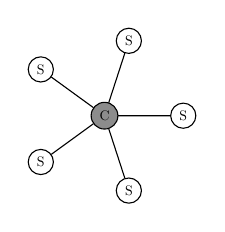
\begin{tikzpicture} [scale=0.5, transform shape]
\tikzstyle{every node}=[draw,shape=circle];
\node [fill = gray!90] (v0) at (0:0) {C};
\node (v1) at ( 0:2) {S};
\node (v2) at ( 72:2) {S};
\node (v3) at (2*72:2) {S};
\node (v4) at (3*72:2) {S};
\node (v5) at (4*72:2) {S};
\draw (v0) -- (v1) % star
(v0) -- (v2)
(v0) -- (v3)
(v0) -- (v4)
(v0) -- (v5);
\end{tikzpicture}
\label{cs}
}  
\subfigure[P2P]  
{  
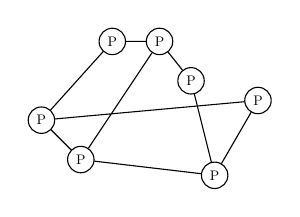
\begin{tikzpicture} [scale=0.5, transform shape]
\tikzstyle{every node}=[draw,shape=circle];
\node (v0) at (0, 2) {P};
\node (v1) at (1, 1) {P};
\node (v2) at (1.8, 4) {P};
\node (v3) at (3, 4) {P};
\node (v4) at (4.4, 0.6) {P};
\node (v5) at (3.8, 3) {P};
\node (v6) at (5.5, 2.5) {P};
\draw (v0) -- (v1)
(v0) -- (v2)
(v0) -- (v6)
(v4) -- (v5)
(v1) -- (v4)
(v2) -- (v3)
(v3) -- (v5)
(v4) -- (v6)
(v3) -- (v1);
\end{tikzpicture}
\label{p2p}
}
\caption{\cs~and P2P architectures}
\end{figure}

Hybrids of {\cs} and P2P exist: Mirrored Game Servers, Distributed Scene Graphs and many more. These architectures are described in~\cite{Ldsg, Scheating, Fgame, Csync}.


% . . . . . . . .  . . . . . . . . . . . . . . . . . . . . . . . . . . . . . . . . . . . . . . . . . . . . . . . . . . . . . . . . . . . . . . . . . . . . . . . . . . . . . . . %
\subsubsection{Synchronization Mechanisms}
\label{syncalgr}

% conservative and optimistic %
The simplest way to maintain consistency among peers is to use totally ordered service, which is often not available. Therefore conservative and optimistic synchronization algorithms have been proposed to prevent or detect (and then correct) misorderings~\cite{Fgame}. 

Conservative synchronization algorithms would allow each peer to process received events only if it is safe to process them. Newly arrived events are usually delayed for an amount of time and the synchronization algorithm can determine the correct execution order. Famous examples are \emph{Chandy-Misra-Bryant algorithm}~\cite{Chandy, Bryant}, \emph{Lockstep synchronization}~\cite{Flockstep} and \emph{fixed time-bucket synchronization}. % Conservative algorithms do not exploit concurrency well and the delay they introduce will reduce interactivity.

Optimistic synchronization algorithms assume received events are in correct order and process them without delay. Then, if late events arrived a \emph{rollback} will be performed and all those optimistically executed events should be canceled and reprocessed. In order to rollback, large memory will used to take multiple snapshots of game state. Also, a mechanism to determine the early bound of rollback (for example the \emph{Global Virtual Time}) will be mandatory. The most famous optimistic synchronization algorithms are: \emph{Time Warp}, \emph{trailing state synchronization}~\cite{Csync}~and \emph{optimistic time-bucket synchronization}~\cite{Doptbkt}.

%------------------------------------------------------------------------------------------------------------------------------------%
\subsection{NDN Background}
\label{ndnbg}

% Basic Exchange %
NDN \emph{names} can be human-readable (for example \url{/Egal/Car/Scene0}). Their binary encodings can be used for routing using longest prefix match.

NDN is designed for content distribution. Two packet types exists in NDN: \emph{Interest} and \emph{Data} (see figure~\ref{packet_types}). A data receiver first initiates an Interest packet that bears the \emph{name} of the \emph{content} it wants. The packet is then routed by name until it reaches a host that has the corresponding content. The matching content object is sent back as a Data packet, satisfying all Interest for it on its way and leaving a trail of `bread crumbs'~\cite{Jndn}~in the routers' memory. Later Interests for the same content may be directly satisfied by the routers. It is guaranteed that in NDN every piece of data would flow through a link for at most once. This would reduce a huge amount of network traffic around content distribution centers.

\begin{figure} 
\begin{center}
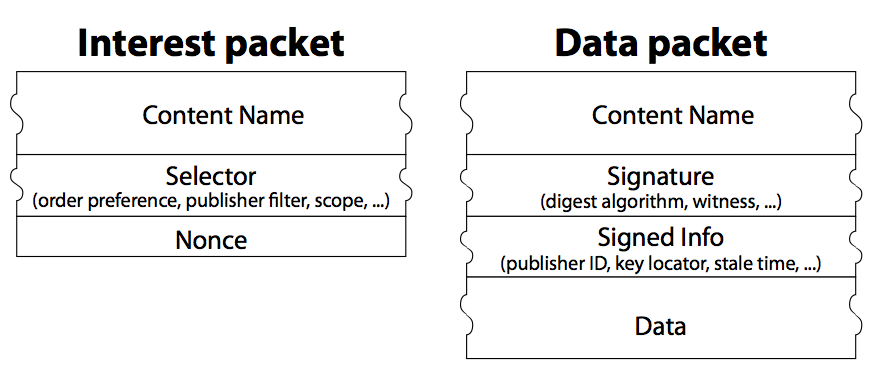
\includegraphics[width=0.4\textwidth] {image/packet_types}
\caption{packet types in NDN}
\label{packet_types}
\end{center}
\end{figure}

Note that NDN is receiver driven. Flow balance is also controlled by the receiver~\cite{Zact}. Also note that multicasting is intrinsically built in.

% . . . . . . . . . . . . . . . . . . . . . . . . . . . . . . . . . . . . . . . . . . . . . . . . . . . . . . . . . . . . . . . . . . . . . . . . . . . . . . . . . . . . . . . %
\subsubsection{CCNx Sync Protocol}
\label{ccnsync}

The CCNx Sync protocol allows applications to define collections of named data in \emph{repositories} that are to be automatically kept in sync with identically defined collections in neighboring repositories~\cite{CCNxSync}. A collection in the repository is also called a \emph{slice}. A local \emph{Sync Agent} builds and manages a \emph{Sync Tree} for a slice, using names that represent the content of the slice. Hashes of Sync Trees are sent among neighboring Sync Agents to detect any discrepancy. Once detected, normal Interest and Data packets will be sent for inconsistent data.

CCNx Sync protocol should not be confused with the game synchronization protocols mentioned in~\nameref{syncalgr}. CCNx Sync maintains data integrity: it keeps local repository slices coherent remote ones. Game synchronization algorithms provide a higher level service: they ensure that sync actions will be taken \emph{in order}.




%===========================================================================%
\section{NDN GAME DESIGN}
\label{gamedesign}


% intro %
% not so sure %
In this section we present game design issues that are specific to NDN games. In most places we use our game adapted from the Unity3D Car Tutorial~\cite{UnityCar} as examples but we are not restricted to this genre.


%------------------------------------------------------------------------------------------------------------------------------------%
\subsection{P2P Game Architecture}

% why did we choose P2P %
We decided that our sample game should be P2P because of the following reasons. First, P2P architectures are scalable and robust, with minimized network latency (see \nameref{game_archi}). Second, these advantages of P2P can be further enhanced by NDN. NDN reduces traffic in the network, which means that given the same bandwidth, more players could join the game. With data packets cached in the network, data receivers will enjoy a even smaller latency. Third, some of the disadvantages of P2P can be (partly) overcame by NDN. Security, for example, will be enhanced by NDN's content validation and trust management scheme. By naming contents instead of hosts, it will be more difficult for attackers to focus on their target. Several types of cheating behavior can be automatically avoided by NDN (see \nameref{discussions}). Finally, improvements on P2P architectures will also benefit the hybrid architectures. As an example, the Mirrored Game Server architecture has its clients connected to a local server, but typically orchestrates its distributed servers into a high-performance P2P network, so NDN could positively affect it in a similar way.


%------------------------------------------------------------------------------------------------------------------------------------%
\subsection{Namespace Design}

% what is a namespace %
Namespace designing is a task specific to NDN application developers. A complete \emph{namespace} of a program is a full collection of names that will be used during the program's execution. Namespace can be presented as trees. For instance, figure~\ref{namespace} is the namespace of our sample car racing game. It is composed of three trees: a \emph{repo tree}, a \emph{network tree} and \emph{game tree}. Each tree node is contains one or more NDN name component(s). One can learn the major functionalities of an application by looking at its namespace design.

\begin{figure}
\begin{center}
\begin{subfigure} [Repo Tree]
{
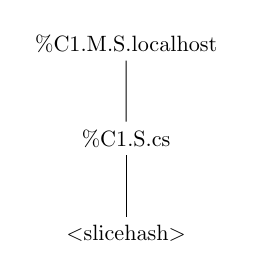
\begin{tikzpicture} [scale=0.8, transform shape]
    %\tikzstyle{every node}=[rectangle,draw]
    \node {\%C1.M.S.localhost}
        child { node {\%C1.S.cs} 
        		child{ node {$<$slicehash$>$} }
        }
       
    ;
\end{tikzpicture}
\label{repo}
}
\end{subfigure}
\begin{subfigure} [Network Tree]
{
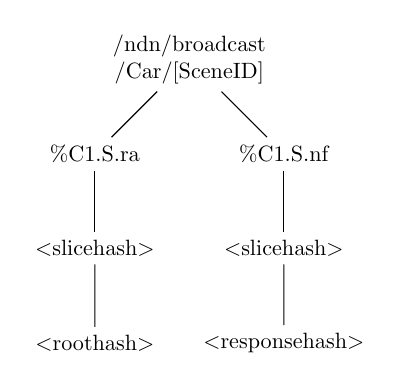
\begin{tikzpicture} [scale=0.8, transform shape]
    \tikzstyle{every node}=[align = center]
    \tikzstyle{level 1} = [sibling distance=30mm]
    \node {/ndn/broadcast \\ /Car/[SceneID]}
        child { node {\%C1.S.ra} 
        		child { node {$<$slicehash$>$} 
			child { node {$<$roothash$>$} }
		}
        }
        child { node {\%C1.S.nf}
        		child { node {$<$slicehash$>$} 
			child { node {$<$responsehash$>$} }
		}
        }
    ;
\end{tikzpicture}
\label{broadcast}
}
\end{subfigure}
\begin{subfigure} [Game Tree]
{
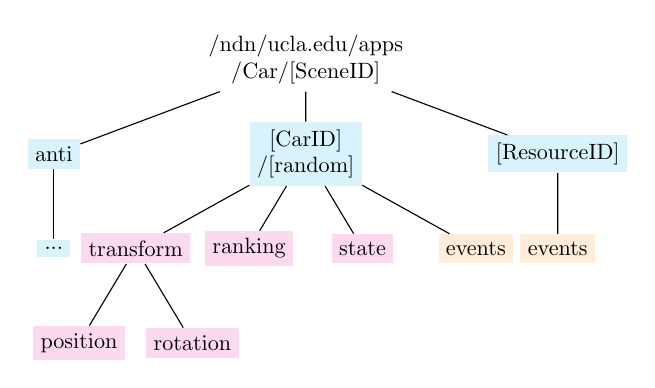
\begin{tikzpicture} [scale=0.8, transform shape]
    \tikzstyle{every node} = [align=center]
    \tikzstyle{asset} = [fill=cyan!15]
    \tikzstyle{state} = [fill=magenta!15]
    \tikzstyle{event} = [fill=orange!15]
    \tikzstyle{level 1} = [sibling distance=40mm]
    \tikzstyle{level 2} = [sibling distance=18mm]
    \node {/ndn/ucla.edu/apps \\ /Car/[SceneID]}
        child{ node [asset] {anti}
        		child { node [asset] {...}}
        }
        child { node [asset] { [CarID] \\ /[random]} 
		child { node [state] {transform} 
			child{ node [state] {position} }
			child{ node [state] {rotation} }
		}
		child { node [state] {ranking} }
		child { node [state] {state} }
		child { node [event] {events} }
        } 
         child { node [asset] {[ResourceID]}
        		child {node [event] {events}} }
        
    ;
\end{tikzpicture}
\label{game}
}
\end{subfigure}
\caption[Caption for LOF]{Namespace of our sample car racing game\footnotemark}
\label{namespace}
\end{center}
\end{figure}
\footnotetext{Colors of the nodes will be explained in \nameref{ase}. Nodes surrounded by $< >$ will be generated at run time using algorithms chosen by NDN. Nodes surrounded by $[ ]$ are variables that will be substituted with multiple values. Note that \slash~are not part of NDN names, they are for illustration purpose only.}


% localhost namespace: repo %
Names in the Repo Tree are used for communication with the local repository: we use CCNx Create Collection Protocol to create a slice, which is a collection of content objects with a common name prefix. Two parameters are used to define the slice: \emph{topo} and \emph{prefix}. They later become the root node of the network tree and the game tree. \url{\%C1.M.S.localhost} restricts the scope to the local node; \url{\%C1.S.cs} is a command marker for the Create Slice Interest~\cite{CCNxCS}. 

% SYNC namespace: [SceneID] %
The network tree illustrates names used by the CCNx Sync Protocol. This protocol is used for name discovery, which explains why its Interests are broadcasted on the NDN testbed (see its root node \url{/ndn/broadcast/...}). Note the use of \url{[SceneID]} in the namespace, which indicates that each scene will have its own slice and be synchronized independently. For small game this may not be necessary; for large games this might be replaced with \url{[DistrictID]} or \url{[BlockID]}. \url{\%C1.S.ra} and \url{\%C1.S.nf} are command markers for the Root Advice Interest and the Node Fetch Interest respectively~\cite{CCNxSync}.

% <nonce> says a lot %
The game tree is most closely related to the object hierarchy in the virtual world. In fact, a big portion of the tree is constructed by extracting objects and their member variables that needs to be transmitted through network. Please note the use of \url{[random]} in the namespace. In a car racing game each car should have a unique identifier in the network, therefore we append a \url{[random]} after \url{[CarID]} to reduce the probability of name collision. \url{[random]} can be omitted only if it is guaranteed by the application that  \url{[CarID]}  would not collide with one another. The same applies to most user-controlled avatars (first person shooters, heroes played by gamers etc.). However, with global virtual resources (such as a potion, a weapon or a bomb) and program controlled avatars (for example a bot enemy), the opposite is the case. The \url{[ResourceID]} in the namespace should never be combined with \url{[random]} and should be named systematically by the application. Otherwise illegal duplications of the resource would plague in the virtual world. 

% namespace for transmission optimization %
The game tree is designed for optimal transmission and does not have to resemble to the game's object hierarchy. In fact, names for immutable objects and static variables almost never appear in the game tree. The reason for excluding immutable objects is quite obvious: they should be \emph{installed} with the software, not \emph{transmitted} through the network. The exclusion of the terrain object in our game tree is a case in point. As for static variables, they should be \emph{initialized} with their parent object (if there is one) and thus can be omitted in many cases. An example for this is our \url{[ResourceID]} node. A resource object in our game has many static members (position, value etc.), which are initialized when the resource is dynamically created. Based on this observation, during synchronization we can pack these constant member variables as a content object and name it after the resource's name. The result is that none of these members become a child node of \url{[ResourceID]} in the game tree. On the other hand, names with little meaning in the virtual world might be added to the game tree just for transmission convenience. The node \url{state}, for example, is not a member variable of the \url{car} class, but a \emph{summary} of all variables under \url{[CarID]/[random]}. 
%In other words, if $transform = \{  \{ x_p, y_p, z_p, t_0\},  \{ x_r, y_r, z_r, t_1\}  \}$ and $ranking = \{  r, t_2\}$, then $state = \{ x_p, y_p, z_p, x_r, y_r, z_r, r, max(t_0, t_1, t_2) \}$. 
Hence, for a peer who is interested in \url{Car0}'s updates, issuing an Interest for the \url{state} is more efficient than sending three packets for \url{position}, \url{rotation} and \url{ranking}.
\footnote{Note that the peer cannot just issue an Interest for \url{car0} and hope to get all the content. An Interest like that will be replied with \url{car0} or one of its children and the peer would not know which child it is until the data packet is received.}

Such name components as \url{state} can have many variations that serve different purposes. For example, an object may want to keep two summaries of different detail levels: a \url{short} summary and a \url{long} summary. The longer summary might interest players who are directly interacting with the object while the shorter one can be used by distant players for the integrity of their global view. Name components can also be \url{public} (for everyone including enemies) or \url{private} (and encrypted, for group members only). An \url{invisible} name component can be used to provide a summary that does not have position information. In effect, this hides a player from others' view. The interesting fact that name components are not restricted to nouns may inspire NDN developers to design namespaces that are rich in meaning and functionalities.




%===========================================================================%
\section{Synchronization}
\label{sync}

The purpose of synchronization is to maintain consistent views of the global game state for all players. The definition of global game state varies from author to author, but it generally means the combined state of all entities (players, non-player characters and objects) in the game. In NDN in particular, the global game state is equivalent to the game tree (figure~\ref{game}) and all its corresponding content objects. Hence, to synchronize a NDN multiplayer on-line game is to synchronize its game tree and all the content objects that underlies.

We divide the problem of synchronizing the game tree into three sub-problems: Asset synchronization, State synchronization and Event synchronization. We recognize nodes in the game tree as \emph{asset}s, \emph{state} and \emph{event}s and use choose different strategies to synchronize them. The idea behind such a division is that assets, state and events have different requirements for synchronization.

%------------------------------------------------------------------------------------------------------------------------------------%
\subsection{Asset, State and Event}
\label{ase}

Asset, state and event are the three classes of content that need to be synchronized. In figure~\ref{game} for example, all asset names are colored blue, all state nodes pink and all event nodes yellow. A formal definition is as follows:
\begin{description*} 
\item [Asset]
A node in the game tree whose presence and absence \emph{cannot} be deduced from the presence and absence of its parent node.
\item [State]
A node in the game tree whose presence and absence \emph{can} be deduced from the presence and absence of its parent node.
\item [Event]
A special State that is defined solely for the interaction among the previous two types.
\end{description*}
Intuitively, the underlying contents will be called \emph{asset}s, \emph{state} and \emph{event}s too and we will not distinguish a content from its name in many cases. Typical examples of assets are those dynamically created entities that do not have a parent in the virtual world: an avatar controlled by a player, a helmet lying on the ground, a bot controlled by game AI. Their corresponding member variables usually fall into the state class: the health points (HP) of an avatar, the defense power of a helmet, and the position of a bot. Actions taken by assets are usually recognized as events: a ``hit'' from an avatar to a bot, a ``heal'' to a group member, a ``pick'' to a public object, or an ``acknowledge as owner'' from an object to a hero. Note that although all these examples have some physical meanings in the virtual world, it is not a prerequisite for any of the three types. Assets, state, and events refer to a broader class of content. This can be exemplified by the \url{anti} asset, which is used to cancel the existence of a character or an object (see \nameref{assetsync} for details).

Asset, state and event are correlated and they model changes and happenings in the virtual world. An asset can change its own state and publish it, but it cannot change the state of another asset or publish the state for that asset. An asset could, however, publish an event that suggests a state change to another asset. The later asset will ``consider'' this suggestion and may change its state correspondingly and publish the new state. The following mini story shows this. Alice was a player-controlled warrior in a role-playing game ``Killing Zombies''. According to our definition Alice is an asset who has a lot of state such as \url{position}, \url{HP} and \url{defense power}. When Alice was walking around searching for zombies, she was voluntarily updating her \url{position} state and publishing it to the network so that other players like \url{Bob} and \url{Trudy} could see her. When she found a zombie (named zombie0), she published a ``hit'' event (\url{.../Alice/events}: \verb|decrease zombie0's HP|). Zombie0 (and other assets) received this event and found itself killed by Alice. So it published a new state saying that its HP has fallen to zero and is going to die. All players within vicinity will get a visual feedback of Alice's ``hit'' event (see \nameref{eventsync} for more details). After killing zombie0, Alice found a prize on the ground. It was a helmet which could increase a warrior's defense power by 20 percent. So Alice published a ``pick'' event (\url{.../Alice/events}: \verb|pick helmet#|) and the helmet published a ``acknowledge as owner'' event in return. The story ends with Alice wearing her new helmet searching for the next zombie. Note that by the end of the story the helmet is not an asset any more since it got a parent object -- Alice. Its original name in the game tree will be ``canceled'' by an anti object and it will become a state (such as \url{.../Alice/outfit/head}).

%We use three different strategies to synchronize assets, state and events. This is based on an observation of their different requirements for consistency. An asset can only be \emph{present} or \emph{absent} in a game tree. They themselves cannot be assigned any value and thus cannot be updated. Once created, there will not be any update about them until they are destroyed. Moreover, all assets are independent entities and the creation and 



%------------------------------------------------------------------------------------------------------------------------------------%
\subsection{Asset Synchronization}
\label{assetsync}

Asset synchronization maintains the consistency of all assets. In the game tree, it is in charge of synchronizing all nodes colored blue. By definition, if all asset names are known then the entire game tree became know, as state and events' existence are predictable. Therefore, asset synchronization is also called \emph{name discovery}.

% . . . . . . . . . . . . . . . . . . . . . . . . . . . . . . . . . . . . . . . . . . . . . . . . . . . . . . . . . . . . . . . . . . . . . . . . . . . . . . . . . . . . . . . %
\subsubsection{An Unordered Mechanism}

% reason for FIFO processing order %
Assets' requirement for consistency is relatively low. Updates about assets can be processed in a FIFO order -- they do not have to be delayed and sorted by their generation time before being processed. The reason comes three folds. First, assets can only be \emph{created} or \emph{destroyed} during their life time. Second, assets are predefined in a game so they will never change once created. The state of an asset will change, but this will not affect the definition of the asset (its name, structure, attributes etc.). Third, by definition, assets are independent of each other. These features make synchronization of assets very similar to synchronizing a directory of files, without caring about the content of those file content.  Files are also dynamic, independent objects whose content can be regarded as merely ``state''s. In file synchronization, the order of which files are added or removed is not important -- as long as a directory shows the right files, it is consistent. The same applies for asset synchronization.

% slice, topo and prefix %
Asset synchronization relies heavily on the CCNx Sync protocol. When a peer initializes its game, the local Sync Agent will write one or more slices into its local repository. These slices are units of synchronization and are defined by \emph{topo} and \emph{prefix}. Topo describes the scope within which the sync function should work. Prefix describes the common semantic location of the slice and its collection of data. For example, our topo is \url{/ndn/broadcast/Egal/Car/[SceneID]} which means the slice is synchronized on the NDN testbed (since its Interests will be broadcasted on it); our prefix is \url{/ndn/ucla.edu/apps/Egal/Car/[SceneID]} which means that this slice is a collection of assets in a scene of a car racing game, which is developed with the Egal library and is one of UCLA's applications running on the NDN testbed. Once the slice is created, the game application can use prefix to name content objects and write them into the local repository. Sync Agent will guarantee the data integrity of the slice with all other identically defined slices within the scope described by topo.

% Adding an asset %
Adding an asset to the game tree corresponds to writing a new content object into the local repository. This content object's name will become a new node in the game tree, and its content usually contains the initialization information of the new asset. Once written into the local repository, this new asset's existence will be announce to all other peers by CCNx Sync. Deleting an existing asset from the name tree corresponds to writing an \emph{anti-asset} into the local repository. An anti-asset has the same name prefix of the deleted asset, but has an extra \url{anti} name component in its name (see figure~\ref{game}). The content of an anti-asset can be defined by the game application. Usually this content is used for anti-cheating and authentication purposes (see~\nameref{discussions}~for details). The existence of an anti-asset will be announced in exactly the same way as a new asset. Note that an anti-asset cannot be deleted. Namely, there should not be anti-anti-asset. 
% Deleting an asset %
% by writing an anti asset
% an anti asset cannot be have an anti asset

A typical example of asset synchronization is player discovery. When a new player joins in the game, its peer will create a new asset node in its local repository. This node represents the player and its content should contain sufficient initialization information such as position, race and class, but it should not contain any private information. Since asset synchronization Interests are broadcasted on the NDN testbed in our sample game (defined by \emph{topo}), the initial information of an asset is know to all players that has the same slice. When a player quits, the game application should first put an anti-player in the local repository before all processes could be terminated. Although the player no longer exists in game logic, its asset and anti-asset information still exists physically in all peers' repository, which is useful for anti-cheating mechanisms (see~\nameref{discussions}). When a player quits unexpectedly (such as due to network failure), s/he would not have a chance to put an anti-player in the local repository. In this case, other peers would query the existence of the player and would eventually write an anti-player for it (see~\nameref{manager}).

% This scheme is unordered
Asset synchronization is unordered. It uses a FIFO order to process all received updates about assets and CCNx Sync Protocol guarantees the data integrity. For instance, if two players $P_1$ and $P_2$ join the game at about the same time (but $P_1$ is slightly earlier than $P_2$), the order of their appearance might vary from peer to peer: from a third peer's view, $P_2$ might appear first if the content object representing $P_2$ reaches the peer earlier. While such phenomena could mean \emph{inconsistency} to some synchronization mechanisms, we find it tolerable, and is in fact beneficial to the game's overall performance. This can be seen from the following comparison. In a conservative synchronization mechanism, when the content object representing $P_2$ arrives at the third peer, it will not be processed until all earlier content arrives. The task of rendering $P_2$ in the virtual world and all tasks after that will be delayed because of the late arrival of $P_1$. If the same thing happens in an optimistic synchronization algorithm, content $P_2$ will be processed but the entire game state will soon rollback when content $P_1$ arrives. After that, all following content objects, including content $P_2$, will be re-processed. In contrast, in our asset synchronization mechanism, no additional delay nor rollback is needed and we eventually produce the same result. The reason why asset synchronization works is that there is no causal relationship between assets, thus different process order does not lead to inconsistency. Note that this should not be confused with state and event synchronization(see~\nameref{statesync}~and~\nameref{eventsync}), in which the process order is critical to consistency maintenance.


% . . . . . . . . . . . . . . . . . . . . . . . . . . . . . . . . . . . . . . . . . . . . . . . . . . . . . . . . . . . . . . . . . . . . . . . . . . . . . . . . . . . . . . . %
\subsubsection{Managing Assets}
\label{manager}
Assets are the only class of active elements that can change the global game state. Hence it is important to manage them in an organized way to prevent spoofing and asset corruption. In a {\cs} architecture this problem is very simple: the central server (group) play the role of central asset manager and all clients are merely renderers that smooth the gameplay. In a pure P2P architecture, however, a clear rule is needed to map assets to the virtual game processes running on each peer. In the rest of this section, we present asset managing rules used in our game scenario. We discuss about various asset managing problems in sections~\nameref{statesync}~and~\nameref{discussions}~to validate these rules.

First of all, an asset must have one \emph{creator} and one \emph{manager}. The creator is a virtual character in the gameplay who \emph{first} directly or indirectly triggers the creation of the asset. The content object written to the repository will be bearing the creator's signature. The manager of an asset is a virtual character selected by the asset creator at creation time to manage the state (and events) of the newly created asset. An object asset's manager and creator must not be the same character. A player asset is his own creator and manager. Only the manager of an asset has the right to produce the asset's anti-asset. In other words, all anti-assets' creator must be the same as the original asset's manager, which also manages the anti-assets.

%The manager of an asset can change but the rules mentioned above shall not be violated. For example, when a player is experiencing an unexpected quit, she can no longer be the manager of herself and those public objects (artifacts, bots etc.) that used to be managed by her. In this case, the public objects 

% every asset has an interaction scope
% the creator chooses a manager for a new asset
% the manager cannot be the creator
% the manager should be far enough from the interaction scope


% . . . . . . . . . . . . . . . . . . . . . . . . . . . . . . . . . . . . . . . . . . . . . . . . . . . . . . . . . . . . . . . . . . . . . . . . . . . . . . . . . . . . . . . %
\subsubsection{Propagation Model and Efficiency}
% relatively slow
% but good for sharing knowledge, good for anti-cheating

The propagation of an asset update is a process of constructing a sink tree in the P2P network, with the asset creator node being that tree's root node (see~\nameref{sinktree}). Since CCNx Sync Protocol works on directly connected peers, data packets propagate in a hop-to-hop manner. Moreover, since all peers in the network can choose the best \emph{face} (connection) to forward its Interest~\cite{Jndn} and the retrieved content will follow the trace of Interest to reach the data receiver, a shortest-path-tree is automatically constructed without the help of any additional calculation.

Because the use of repository in CCNx Sync, asset synchronization is relatively slower than state synchronization and event synchronization. However, CCNx Sync also forms a solid base of sharing knowledge about the entire game tree, which is vital to the virtual world's evolvement. Given the fact that assets do not generate as much updates as state and events do, we conclude that the advantages of using CCNx Sync outweighs the disadvantages.

\begin{figure}
\begin{center}
\begin{subfigure} []
{
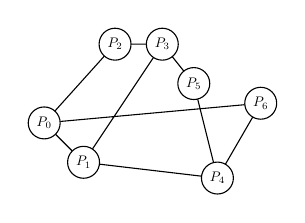
\begin{tikzpicture} [scale=0.5, transform shape]
\tikzstyle{every node}=[draw,shape=circle];
\node (v0) at (0, 2) {$P_0$};
\node (v1) at (1, 1) {$P_1$};
\node (v2) at (1.8, 4) {$P_2$};
\node (v3) at (3, 4) {$P_3$};
\node (v4) at (4.4, 0.6) {$P_4$};
\node (v5) at (3.8, 3) {$P_5$};
\node (v6) at (5.5, 2.5) {$P_6$};
\draw (v0) -- (v1)
(v0) -- (v2)
(v0) -- (v6)
(v4) -- (v5)
(v1) -- (v4)
(v2) -- (v3)
(v3) -- (v5)
(v4) -- (v6)
(v3) -- (v1);
\end{tikzpicture}
}
\end{subfigure}
\begin{subfigure}[]
{
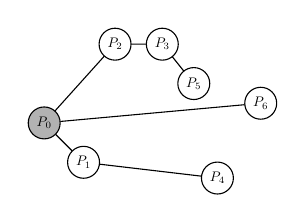
\begin{tikzpicture} [scale=0.5, transform shape]
\tikzstyle{every node}=[draw,shape=circle];
\node [fill=black!30] (v0) at (0, 2) {$P_0$};
\node (v1) at (1, 1) {$P_1$};
\node (v2) at (1.8, 4) {$P_2$};
\node (v3) at (3, 4) {$P_3$};
\node (v4) at (4.4, 0.6) {$P_4$};
\node (v5) at (3.8, 3) {$P_5$};
\node (v6) at (5.5, 2.5) {$P_6$};
\draw (v0) -- (v1)
(v0) -- (v2)
(v0) -- (v6)
%(v4) -- (v5)
(v1) -- (v4)
(v2) -- (v3)
(v3) -- (v5)
%(v4) -- (v6)
%(v3) -- (v1)
;
\end{tikzpicture}
}
\end{subfigure}
\caption{Sink Tree Propagation}
\label{sinktree}
\end{center}
\end{figure}


%------------------------------------------------------------------------------------------------------------------------------------%
\subsection{State Synchronization}
\label{statesync}
% Task: sync the red nodes
% The state of an asset can only be published by its manager
% what about global state? **** Oh! ****
State synchronization maintains the consistency of the state of all assets. In figure~\ref{game}, state synchronization is in charge of synchronizing all nodes and corresponding content objects colored pink. State synchronization differs from asset synchronization in that it does not use CCNx Sync and it does not processes state updates in their arrival order.


% . . . . . . . . . . . . . . . . . . . . . . . . . . . . . . . . . . . . . . . . . . . . . . . . . . . . . . . . . . . . . . . . . . . . . . . . . . . . . . . . . . . . . . . %
\subsubsection{An Ordered Mechanism with Misses}
\label{orderedmiss}
% why state should be in the right order %
State synchronization should be ordered. When a peer receives a state update, the effect of this update will last until the next update comes. Moreover, state tend to be correlated, thought not necessarily causal. For example, a character's state change in position tend to be limited (by the maximum speed of that character), but if state updates were processed out of order, it will produce chaos at the receivers' end. In NDN in particular, processing state packets according to their generation time is especially important. This is because a series of state updates usually share the same name, and all of them will be stored in the network cache for future use. If state synchronization were unordered, NDN receivers could receive some randomly-old matching content, making the synchronization mechanism useless.

% how does the mechanism work: everyone registers for "state" of everyone
% increasing exclusion filter guarantees the right order
% rightmost child guarantees to get the freshest state, but might cause state miss
In state synchronization each peer plays both the role of \emph{publisher} and \emph{audience}. Each player (asset manager) publishes his/her own state (and the state of all assets under his/her management) and listens to state updates of other assets. Only asset managers have the right to publish new state of the assets under its management. The published state will bear the manager's signature and all spoofing will be detected immediately since every peer in the network is aware of the asset-manager bounding -- it is written in every peer's repository. A player listen to state updates by keeping an outstanding interest for each distinct state names. By dynamically adjusting his/her interest pool, a player decides whose state s/he wants to follow and how detailed the state updates should be. For example, every player would probably issue interests for all other players' \url{position} state. Although some players might be out of sight, it is good to know where everyone is to have a global view of the game. Moreover, by keeping track of all participants position, a player would be notified when some other player is approaching and would probably issue interests for more a detailed state of the approacher (\url{rotation}, \url{type} just to name a few).

The correct process order of state synchronization is guaranteed by the use of an \emph{exclusion filter} in the Interest packet. An exclusion filter is a of \emph{Selector} in an Interest packet (see figure~\ref{packet_types}). It is used to exclude certain content objects whose names match the name of the Interest packet. When a received state update has been processed, the timestamp in the Data packet, which marks the generation time of that state, will be extracted. This timestamp will be used as the lower bound of the generation time of the next wanted state. This non-decreasing timestamp lower bound guarantees that all received packets are already automatically sorted according to their generation time. It also guarantees that no duplicate state will be received.

Since state can be dated easily, we put another selector \url{RightmostChild} in the Interest packet. This will select the latest version of available state, the rightmost child in the name tree, thus guaranteeing the freshness of every state received.
% why state can be missed: one will only miss other's state, which will be updated soon%
% events will not be missed, if an asset really cares that much about another asset's state, it can gather all events and check by himself %

It is guaranteed in state synchronization that all states will be processed in order, but it is not guaranteed that there will not be any state missing. On the contrary, because state synchronization does not introduce delay or perform rollback, there must be some state missing from time to time. But, the problem is how does such kind of state miss affect game state consistency. Note that a state is not a \emph{log of changes} from an asset's old value to its new value. A state is a \emph{snapshot} of the value specified by the state name. Hence, if a state failed to reach a peer (because that peer has increased its lower bound of timestamp), then its content must have either been dated or included in the state generated later. Also note that state changes will not have any causal effects either. They do not lead to any change -- no asset change, no state change, no event generation. State is the \emph{result}, and will never be the \emph{cause}. State is published by one authenticated publisher and is published just to help its audiences to have a knowledge of the happenings within the game play. Therefore we conclude that the missing in state synchronization will not hurt consistency, and introducing extra delay with a lockstep mechanism or with rollback mechanism is unnecessary.


% . . . . . . . . . . . . . . . . . . . . . . . . . . . . . . . . . . . . . . . . . . . . . . . . . . . . . . . . . . . . . . . . . . . . . . . . . . . . . . . . . . . . . . . %
\subsubsection{Bandwidth Consumption}
% state generates the most traffic
% interests aggregate
% content propagate
State synchronization generates the largest amount of packets among the three types of synchronization. Every manager should periodically publish new state for all its managed assets, otherwise the manager (or the player) would be suspected as unconnected by other peers and eventually be kicked out. In addition to these regularly published states, managers should also promptly publish new state when there is a major change in the asset values. But what really creates traffic is the need at the receivers' end. Typically in a P2P game, all player would want to learn some basic information of all other players (such as the much needed \url{position} state mentioned in section~\nameref{orderedmiss}). So if a network has $N$ peers, every state update cycle there will be at least $2(N-1)^N$ packets going on to request and send data about state updates. This pompous amount of packets would render any P2P game on IP network unscalable. On NDN however, such kind of congestion will be largely alleviated. NDN guarantees that every packet will go through a link for at most once. Interests issued by state audiences will aggregate locally. Only one Interest will be sent out further to retrieve the matching state content. When the state content is retrieved, all Interests pending at a local node or router will be satisfied. In this way, P2P games can grow to a much larger scale than it could on the IP network.

% . . . . . . . . . . . . . . . . . . . . . . . . . . . . . . . . . . . . . . . . . . . . . . . . . . . . . . . . . . . . . . . . . . . . . . . . . . . . . . . . . . . . . . . %
\subsubsection{Distribution Efficiency}
% all interests pending
% efficiency higher than asset sync

State is also propagated following the branches of a sink tree, but the distribution efficiency of state synchronization is significantly higher than that of asset synchronization. First, all peers keep their interest for state updates \emph{outstanding}. In other words, peers will always keep a pending Interest for each state they want. Once a new state is published, it will quickly propagate from the publisher to all its audiences. This is not like asset synchronization where Sync Agents has to spend some extra time to learn about a neighboring slice's difference. Asset synchronization is an efficient fast-forwarding strategy with little delay brought by the intermediate nodes. Second, asset synchronization does not utilize peers' repository, which further improves its distribution efficiency.

%------------------------------------------------------------------------------------------------------------------------------------%
\subsection{Event Synchronization}
\label{eventsync}
% Task: to synchronize the yellow nodes
Event is a special type of state. It is similar to state in that it can be deduced from its parent and can only be published by an authenticated manager. % **** Oh! ****%
However, the differences are more significant: events can lead to state changes and event asset changes. In fact, they are designed to produce changes.

Event synchronization is an ordered synchronization mechanism with no potential misses. In figure~\ref{game}, event synchronization is in charge of all nodes and corresponding content objects colored yellow.
% events is a special type of state
% Only the manager could publish events


% . . . . . . . . . . . . . . . . . . . . . . . . . . . . . . . . . . . . . . . . . . . . . . . . . . . . . . . . . . . . . . . . . . . . . . . . . . . . . . . . . . . . . . . %
\subsubsection{An Ordered Mechanism with No Miss}
% why events should be ordered: hit and heal
% why there should be no miss: heal and hit
Events should be processed according to their generation time and no event should be missed. To see this, one can imagine that if there were two events \url{hit} and \url{heal}, targeting at Bob, a brave hero who has only the smallest amount of HP left, different process order could lead to different states: if \url{hit} is processed first, the following \url{heal} event would be helpless because Bob would have already died by then; if \url{heal} is processed first, then Bob might still have chance to live and fight. A similar example would show why there should not be any event misses: if the \url{heal} event was indeed generated earlier than the \url{hit} event, but unfortunately was missed by Bob because he has updated his lower bound for timestamp, Bob is throwing away his own chances of living.


% how do we ensure that there is no miss? we use sequence number
Event synchronization mechanism evolves from the state synchronization mechanism. We require event publishers to add sequence numbers to each published event. The receiver still uses an exclusion filter to avoid getting duplicated events, but will only update its exclusion filter when the received event has the correct sequence number. If not, the event receiver would notice the events missing and should keep its lower bound of timestamp intact.

% but then, the order is broken, so we rollback when necessary
Such mechanism means that if a late event arrived, it will still be processed. (Unlike state synchronization mechanism, in which all late state are directly ignored.) We do not introduce delay to wait for a late event, instead, we let an asset optimistically executes the received events, assuming all late events are not targeted at it. When a late event was targeting at the asset however, we perform a rollback to the asset's earlier state. The asset's state should be rolled back to the state just before the generation time of the late event, and all events after that should be re-executed. 

% what is the earliest time an asset should rollback? Local Virtual Time
To be able to perform rollbacks each asset manager must manage a state history of all assets under its management. An important problem to take into consideration is to determine the earliest time to which a rollback could happen. This time is called the \emph{Local Virtual Time} and can be calculated by searching through all exclusion filters of the asset's event Interests and finding out the earliest bound in those exclusion filters. Put simply, the Local Virtual Time separates an asset's timeline into two sections: the section before the Local Virtual Time is known to be consistent; the section after the Local Virtual Time has events that are optimistically executed and is subject to rollback.

% A critical event is an event that causes asset change
% writing the anti asset should be delayed
Events generally causes state changes, but sometimes they can also cause asset changes. Events that leads to asset changes are called \emph{critical event}s. For example, a \url{hit} event would usually only decrease a hero's HP, but it could also lead to a hero's death if the attacking power was too strong or if the hero's HP was already too low. When merely causing HP decrease, the \url{hit} event is a normal event; when causing a hero's death, the \url{hit} event becomes a critical event. Another typical example of critical events is the \url{acknowledge as owner} event published by objects, which would lead to the cancellation of the object's name in the game tree. 

When a critical event happens, its resulting asset change should be delayed for a brief amount of time to prevent unnecessary overheads caused by potential rollback. For example, if Bob received a \url{hit} event which turned out to be a critical event for him, the manager of Bob should plan to write an \url{.../anti/Bob} into its local repository but it does not have to do it in haste. An advice to the manager is to wait until the Local Virtual Time has evolved to be some value later than the timestamp of the critical event. If no \url{heal} event arrives during this delay period, then the proposed anti-asset can be written. But if a \url{heal} does arrive, Bob's state will be rolled back to the state before the timestamp of \url{heal} and all events after that, including the \url{hit} event, should be re-executed.

%------------------------------------------------------------------------------------------------------------------------------------%
\subsection{A Comparison with the Time Warp}






%===========================================================================%
\section{IMPLEMENTATION}
\label{implementation}
\def\tm{\leavevmode\hbox{$\rm {}^{TM}$}} %注册符 网上找的

We implemented asset, state and event synchronization in both C and C\#. We organize these functions in our \emph{Egal} library which can be reused by future programers. Moreover, we wrapped the Egal library as a Unity3D\tm~Pro plugin so that it can provide some direct support for Unity\tm~programmers. Last but not least, we adapted Unity\tm's Car Racing Tutorial~\cite{UnityCar}~into a P2P multiplayer on-line game running over NDN.





%===========================================================================%
\section{DISCUSSIONS}
\label{discussions}

%------------------------------------------------------------------------------------------------------------------------------------%
\subsection{Bandwidth Consumption}

%------------------------------------------------------------------------------------------------------------------------------------%
\subsection{Scalability}

%------------------------------------------------------------------------------------------------------------------------------------%
\subsection{Security}
% attacking will be harder, since it's difficult to target
Thanks to NDN, network security for games is enhanced. Spoofing has become more difficult, as NDN requires all content packets to be signed. Attacking a specific host will be much more difficult than it was before, since NDN does not talk about hosts, but about contents, so attackers will find it hard to direct their packets to their target.

%------------------------------------------------------------------------------------------------------------------------------------%
\subsection{Cheating Avoidance}
%Trudy claims that she picked the helmet but the helmet didn't say so: when anti helmet was written into the repo, its content object should be "I was picked by Alice"

% Trudy publishes other untrue state: "Bob healed me, so my HP should increase" --

% " I just killed zombie0 so my Gold should increase" -- similar to our helmet's case

Content objects representing assets have the extra functionality of preventing cheating besides providing initialization information for new assets. The fact that these content objects will remain static in every peer's local repository should be exploited for optimal use. One example utilizing these content to prevent cheating involves binding assets with their managers by writing such bound as the data of an asset name. In this way, all state and event updates received can be easily authenticated by individual peers since the whole mapping from assets to their managers is stored in the synchronized repository. 

Content of anti-assets can also be used to prevent spoofing in some cases. The destruction of an asset often bring benefits to some players. For example, the destruction of a helmet often means that some player has picked it, and the destruction of a zombie often means that some player's experience has increased. To prevent players from spoofing, such as claiming that they have just killed a zombie while they have actually not done so, we can quote or write the critical event that directly causes the an asset's destruction in the content data of the anti-asset. Since anti-assets are propagated and stored throughout the network just as assets are, the spoofing behavior mentioned above will soon be detected. 




%===========================================================================%
\section{RELATED WORK}
\label{relatedwork}



%===========================================================================%
\section{CONCLUSIONS}
\label{conclusions}







%===========================================================================%
\section{ACKNOWLEDGEMENTS}




%===========================================================================%
\balance
% If you want to use smaller typesetting for the reference list,
% uncomment the following line:
% \small
\bibliographystyle{acmsigchi}
\bibliography{sample}
\end{document}
